%%%%%%%%%%%%%%%%%%%%%%%%%%%%%%%%%%%%%%%%%
% Beamer Presentation
% LaTeX Template
% Version 1.0 (10/11/12)
%
% This template has been downloaded from:
% http://www.LaTeXTemplates.com
%
% License:
% CC BY-NC-SA 3.0 (http://creativecommons.org/licenses/by-nc-sa/3.0/)
%
%%%%%%%%%%%%%%%%%%%%%%%%%%%%%%%%%%%%%%%%%

%----------------------------------------------------------------------------------------
%	PACKAGES AND THEMES
%----------------------------------------------------------------------------------------

\documentclass{beamer}

\mode<presentation> {

% The Beamer class comes with a number of default slide themes
% which change the colors and layouts of slides. Below this is a list
% of all the themes, uncomment each in turn to see what they look like.

\usetheme{default}
%\usetheme{AnnArbor}
%\usetheme{Antibes}
%\usetheme{Bergen}
%\usetheme{Berkeley}
%\usetheme{Berlin}
%\usetheme{Boadilla}
%\usetheme{CambridgeUS}
%\usetheme{Copenhagen}
%\usetheme{Darmstadt}
%\usetheme{Dresden}
%\usetheme{Frankfurt}
%\usetheme{Goettingen}
%\usetheme{Hannover}
%\usetheme{Ilmenau}
%\usetheme{JuanLesPins}
%\usetheme{Luebeck}
%\usetheme{Madrid}
%\usetheme{Malmoe}
%\usetheme{Marburg}
%\usetheme{Montpellier}
%\usetheme{PaloAlto}
%\usetheme{Pittsburgh}
%\usetheme{Rochester}
%\usetheme{Singapore}
%\usetheme{Szeged}
%\usetheme{Warsaw}

% As well as themes, the Beamer class has a number of color themes
% for any slide theme. Uncomment each of these in turn to see how it
% changes the colors of your current slide theme.

%\usecolortheme{albatross}
%\usecolortheme{beaver}
%\usecolortheme{beetle}
%\usecolortheme{crane}
%\usecolortheme{dolphin}
%\usecolortheme{dove}
%\usecolortheme{fly}
%\usecolortheme{lily}
%\usecolortheme{orchid}
%\usecolortheme{rose}
%\usecolortheme{seagull}
%\usecolortheme{seahorse}
%\usecolortheme{whale}
%\usecolortheme{wolverine}

%\setbeamertemplate{footline} % To remove the footer line in all slides uncomment this line
\setbeamertemplate{footline}[page number] % To replace the footer line in all slides with a simple slide count uncomment this line

\setbeamertemplate{navigation symbols}{} % To remove the navigation symbols from the bottom of all slides uncomment this line
}

\usepackage{graphicx} % Allows including images
\usepackage{booktabs} % Allows the use of \toprule, \midrule and \bottomrule in tables
\usepackage{color}
\usepackage{listings}
\lstset{
	columns=flexible,
	keepspaces=true,
	showstringspaces=false,
	commentstyle=\color{gray},
	keywordstyle=\color{purple},
	stringstyle=\color{green}
}

%----------------------------------------------------------------------------------------
%	TITLE PAGE
%----------------------------------------------------------------------------------------

\title[Short title]{Will a business close?} % The short title appears at the bottom of every slide, the full title is only on the title page

\author{Yuxiang Gong} % Your name
\institute[] % Your institution as it will appear on the bottom of every slide, may be shorthand to save space
{
	
\includegraphics[width=.35\textwidth]{closed}
 % Your institution for the title page
\textit{} % Your email address
}
\date{August 20, 2019} % Date, can be changed to a custom date

\begin{document}

\begin{frame}
\titlepage % Print the title page as the first slide
\end{frame}

\begin{frame}
\frametitle{Overview} % Table of contents slide, comment this block out to remove it
\tableofcontents % Throughout your presentation, if you choose to use \section{} and \subsection{} commands, these will automatically be printed on this slide as an overview of your presentation
\end{frame}

%----------------------------------------------------------------------------------------
%	PRESENTATION SLIDES
%----------------------------------------------------------------------------------------

%------------------------------------------------
\section{Project Description} % Sections can be created in order to organize your presentation into discrete blocks, all sections and subsections are automatically printed in the table of contents as an overview of the talk
%------------------------------------------------
\begin{frame}
\frametitle{Project Description}

\begin{figure}
	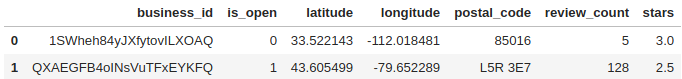
\includegraphics[width=.95\textwidth]{business_head}
\end{figure}

%\begin{center}
%	\begin{tabular}{|c|c|c|}
%	\hline
%			& open & closed \\
%	\hline
%	Counts	&  158525 & 34084 \\
%	\hline
%	\end{tabular} 
%\end{center}

In the business dataset, about 18\% of businesses have closed. This project is going to get insights into Yelp's datasets to find the answers to the following questions:
\vspace{1em}
\begin{itemize}
	\item What could be the factors lead to the closure of a business?
	\item Can we predict if a business will stays open or closes in the near future?
\end{itemize}
\begin{block}{Idea:}
	Take the \textcolor{blue}{is\_open} (1, 0) feature in the business dateset as the label, collect features to build a binary classification model.
\end{block}

\end{frame}

%\subsection{Subsection Example} % A subsection can be created just before a set of slides with a common theme to further break down your presentation into chunks

%------------------------------------------------
\section{Feature Engineering}
%------------------------------------------------
\subsection{Review and Check-in Information}

\begin{frame}
\frametitle{Review Information}

\begin{figure}
	\centering
	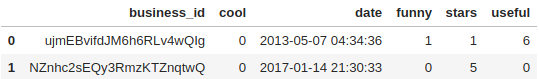
\includegraphics[width=.75\textwidth]{review_head}
\end{figure}
The review data contains unique Id of businesses and users, text comments, comments entry time, stars and votes from other users. This project focuses on numerical data, thus the following features to each business are extracted:
\vspace{1em}
\begin{itemize}
	\item Total number of \textcolor{blue}{cool}, \textcolor{blue}{funny} and \textcolor{blue}{useful} votes 
	\item Number of reviews per month
	\item Duration of reviews in years (i.e. time interval between first time and latest comments)
	\item Year and month of first and latest comments
\end{itemize}

\end{frame}

\begin{frame}
\frametitle{Check-in Information}
\begin{figure}
	\centering
	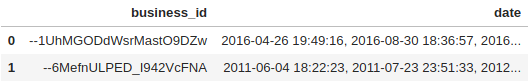
\includegraphics[width=.72\textwidth]{checkin_head}
\end{figure}
There are certain discounts to the users if they check-in a business on Yelp, which could be a detector of how much a business devotes to attract customers. The check-in dataset contains business Id and time points of check-in. Time related features are extracted:
\vspace{1em}
\begin{itemize}
	\item Total number of check-ins
	\item Check-ins per month
	\item Duration of check-ins in years
	\item Year and month of first and latest check-ins
\end{itemize}
\end{frame}

\subsection{Enrich Features - population, land area, household income}
\begin{frame}
\frametitle{Enrich Features}
Normally, a business is closely related to the residents around. However, Yelp can't provide these information. Thanks to \textbf{uszipcode}, a database which contains various features like geography, demographics, income in USA which can be searched via postal code, address and geographic coordinates.\vspace{1em}

In this project, the postal code is used to acquire statistics about residents around businesses in US, following information are obtained:\vspace{1em}
\begin{itemize}
	\item Population and population density
	\item Land area
	\item Median household income
\end{itemize}

The number of businesses is reduced after searching through postal code in the US (from 192609 to 96632).
\end{frame}

\subsection{Location Clustering}
\begin{frame}
\frametitle{Location Clustering}
Apart from the local residents, the density of businesses might also play a crucial role in running a business. The latitude and longitude coordinates can be used to determine if a business is in a chain ($>$5) or not.\vspace{1em}

The DBSCAN (Density-Based Spatial Clustering of Applications with Noise) algorithm is used to cluster the businesses according to their latitude ($\varphi$) and longitude ($\lambda$). The distance are calculated with haversine formula:
\begin{equation*}
	hav(\Theta) = hav(\varphi_2 -\varphi_1) + cos(\varphi_1)cos(\varphi_2)hav(\lambda_2 - \lambda_1),
\end{equation*} 
where $\Theta = \dfrac{d}{r}$, d- spherical distance, r- radius of the earth.

\end{frame}

\begin{frame}
\frametitle{Location Clustering}
If the minimum distance between two businesses is within 50 meters, the businesses are clustered in a group. Here is the result of a cluster in Pittsburgh, PA. There are 171 businesses (35 \textcolor{red}{closed} and 136 \textcolor{blue}{open}) on the same street, which are supposed in a chain. 

\begin{figure}
	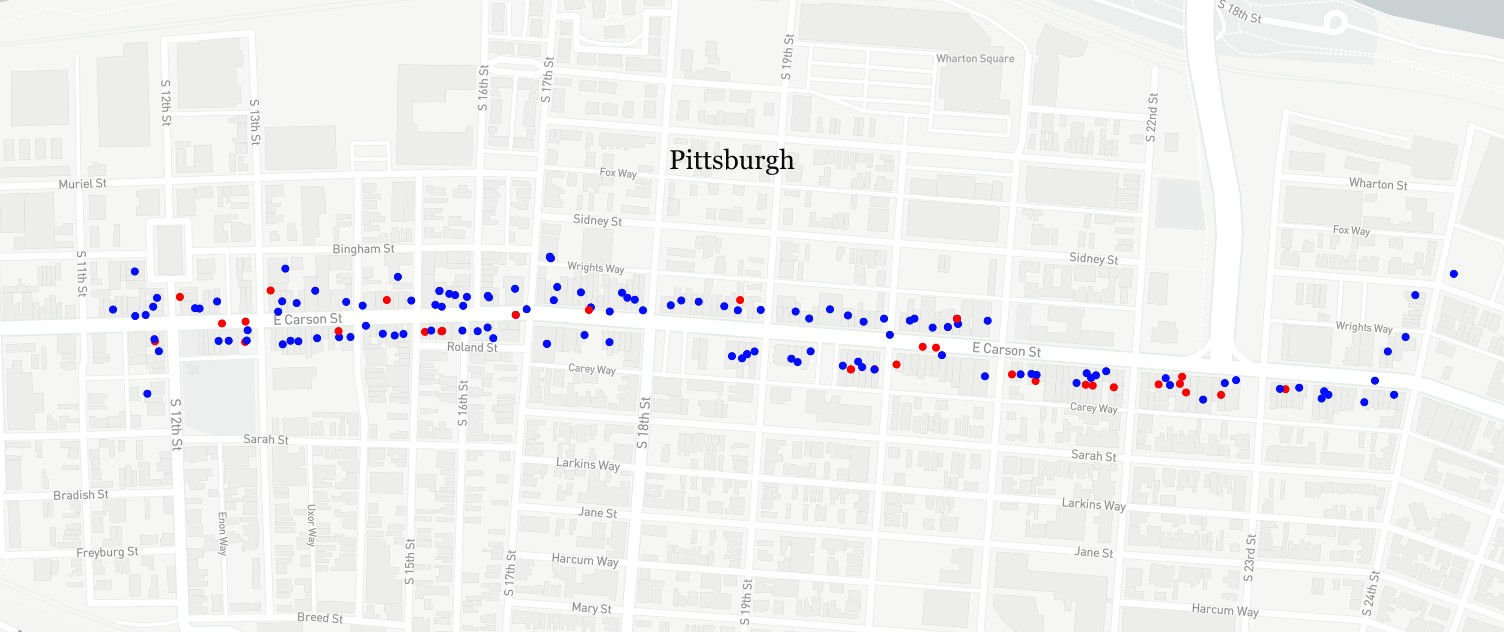
\includegraphics[width=\textwidth]{Pittsburgh.jpg}
\end{figure}

\end{frame}

%------------------------------------------------
\section{Machine Learning Model}
%------------------------------------------------
\subsection{Sampling}
\begin{frame}
\frametitle{Sampling}
The number of closed businesses is about 15\% after feature engineering, which would cause over-fitting on the open businesses due to the imbalanced datasets. The solution is to oversampling the closed businesses to comparable amount of the open businesses. \vspace{1em}


\begin{columns}
	\column{0.5\textwidth}
	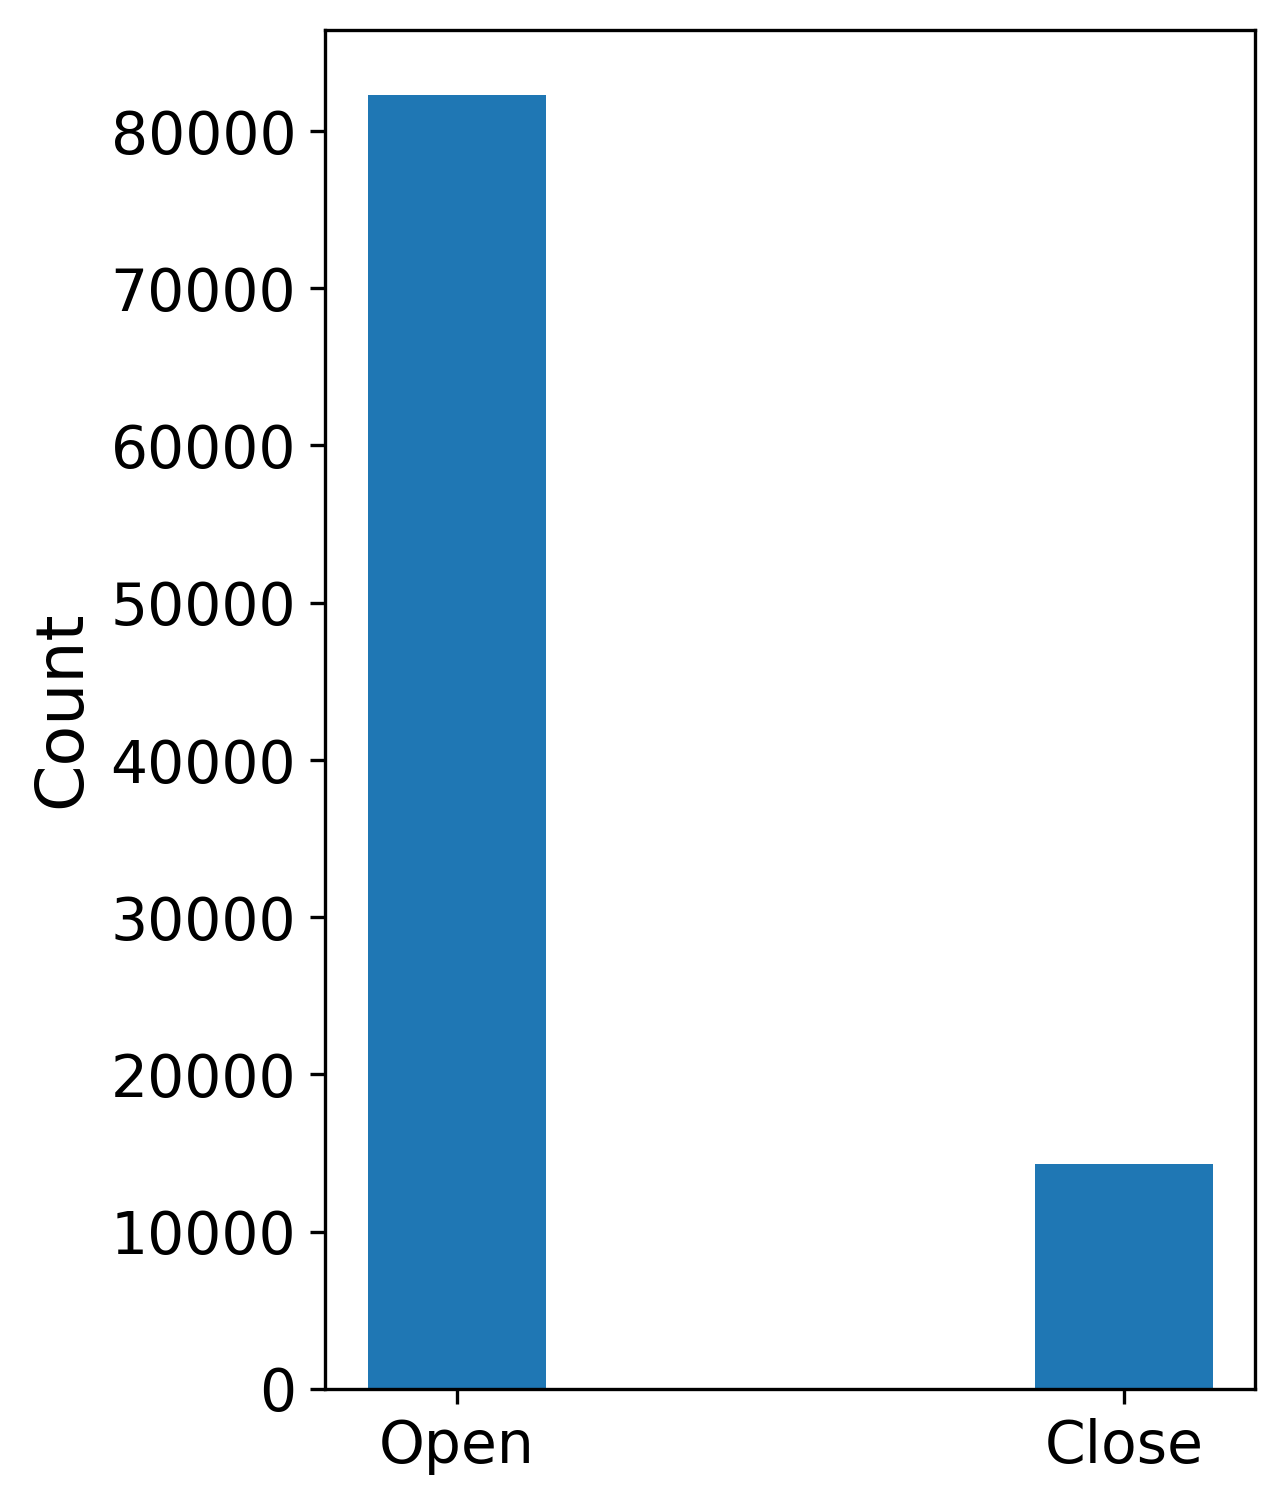
\includegraphics[width=.9\textwidth]{open_close_count}
	\column{0.5\textwidth}
	\begin{itemize}
		\item Split training and  testing data (33\%)
		\item Randomly oversampling the closed businesses in the training set to 80\% of the open businesses
	\end{itemize}
\end{columns}

\end{frame}
\subsection{Model Selection}
\begin{frame}
\frametitle{Model Selection}
The features like population, year, cluster labels are in different scales, thus a model which is not sensitive to the scale is preferred. Among the commonly used algorithms for binary classification, lightGBM, Random Forests and Logistic Regression are employed. Here is the performance in ROC curves. \textbf{lightGBM} has the best performance.
\begin{figure}
	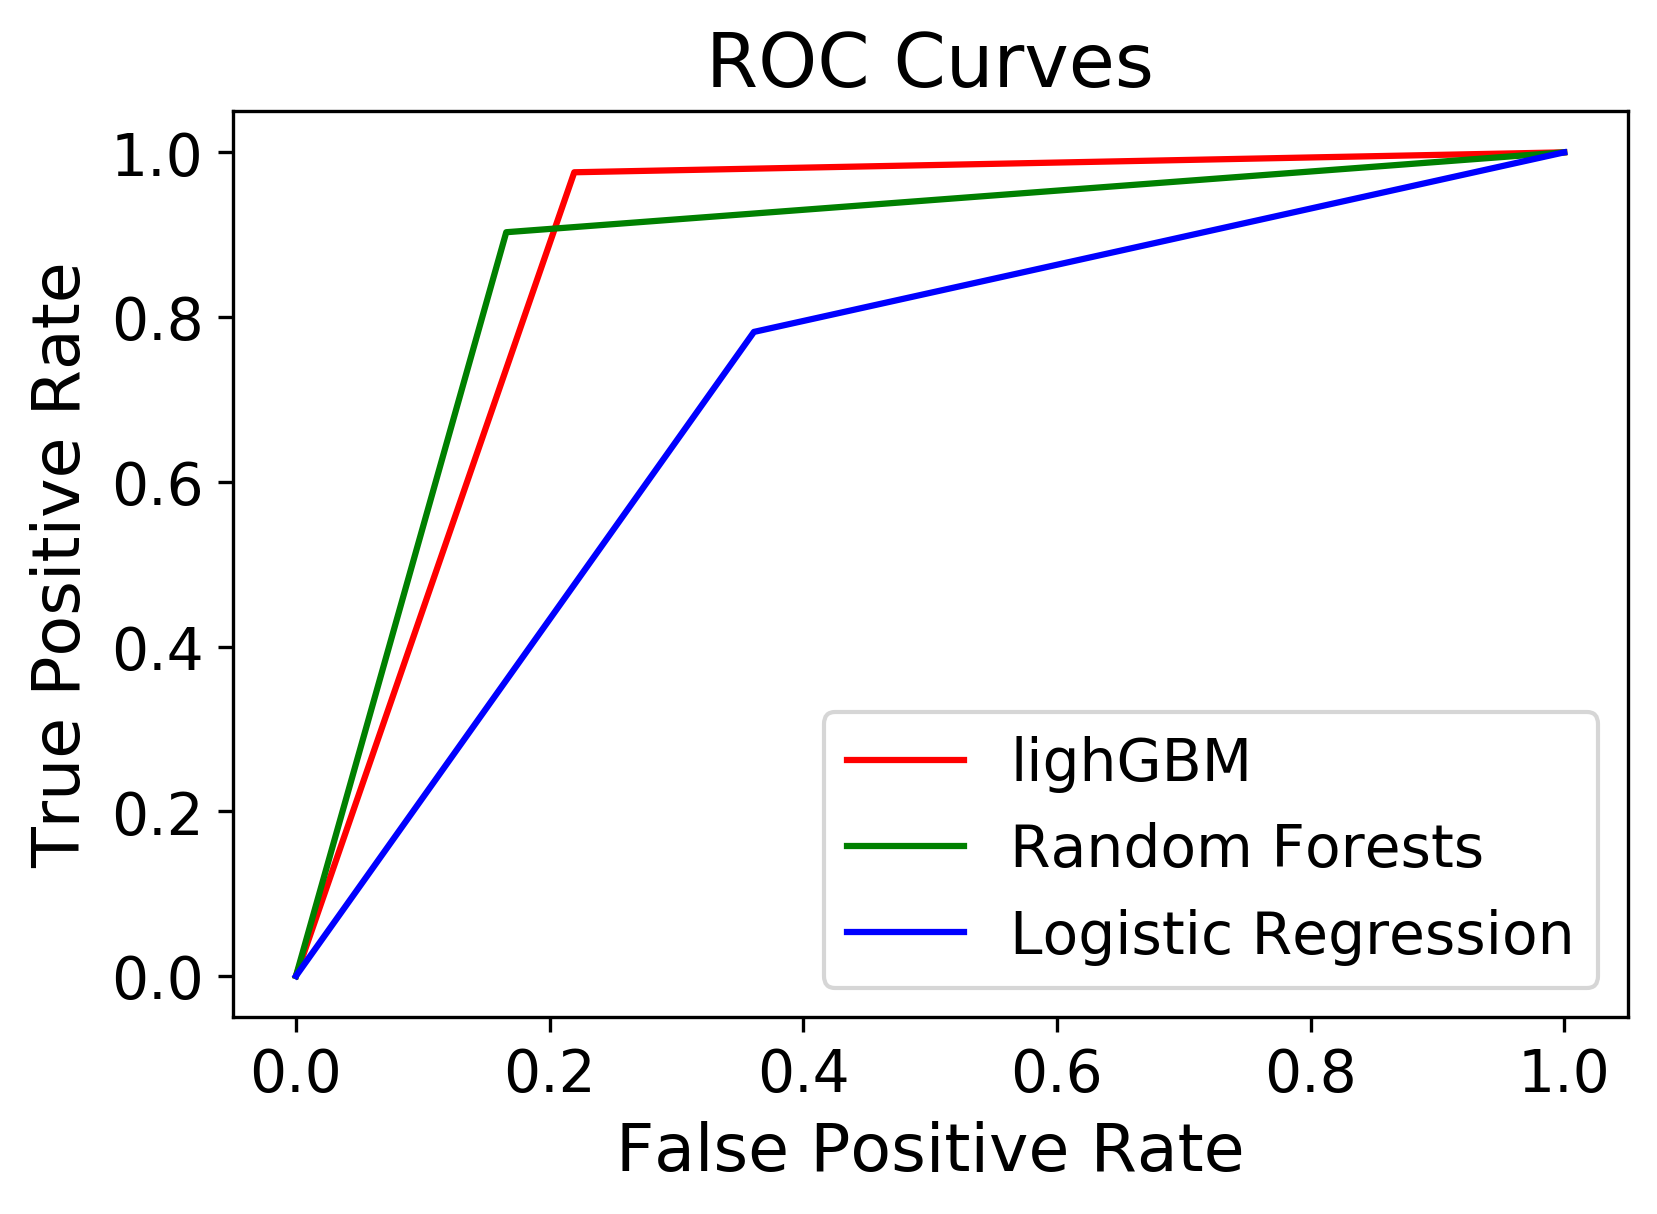
\includegraphics[width=.65\textwidth]{roc}
\end{figure}

\end{frame}
\subsection{Model Training}
\begin{frame}[fragile]
\frametitle{Model Training}
The sampled training data is passed to lightGBM, and the prediction is made with the testing data. \vspace{1em}

The hyperparameters are tuned with RandomizedSearchCV, with the scoring metric as recall. The function can be activated by assigning  \underline{tune\_parameters=True} while running the code.\vspace{1em}

\begin{lstlisting}
	# run model training
	model.main(df_business, tune_parameter=False)
\end{lstlisting}
\end{frame}
%------------------------------------------------
\section{Results and Insights}
%------------------------------------------------
\subsection{Performance}
\begin{frame}
\frametitle{Performance}
Overall accuracy: 94.42\%
\begin{tabular}{cl}  
	\begin{tabular}{|c|c|c|}
	\hline
	& open & closed \\
	\hline
	Precision	& 0.96   & 0.87 \\
	\hline
	Recall &0.98  &0.77 \\
	\hline
	f1-score &0.97  &0.82 \\
	\hline
	Support &23192  &4475 \\
	\hline
\end{tabular} 
&
\begin{tabular}{c} 
	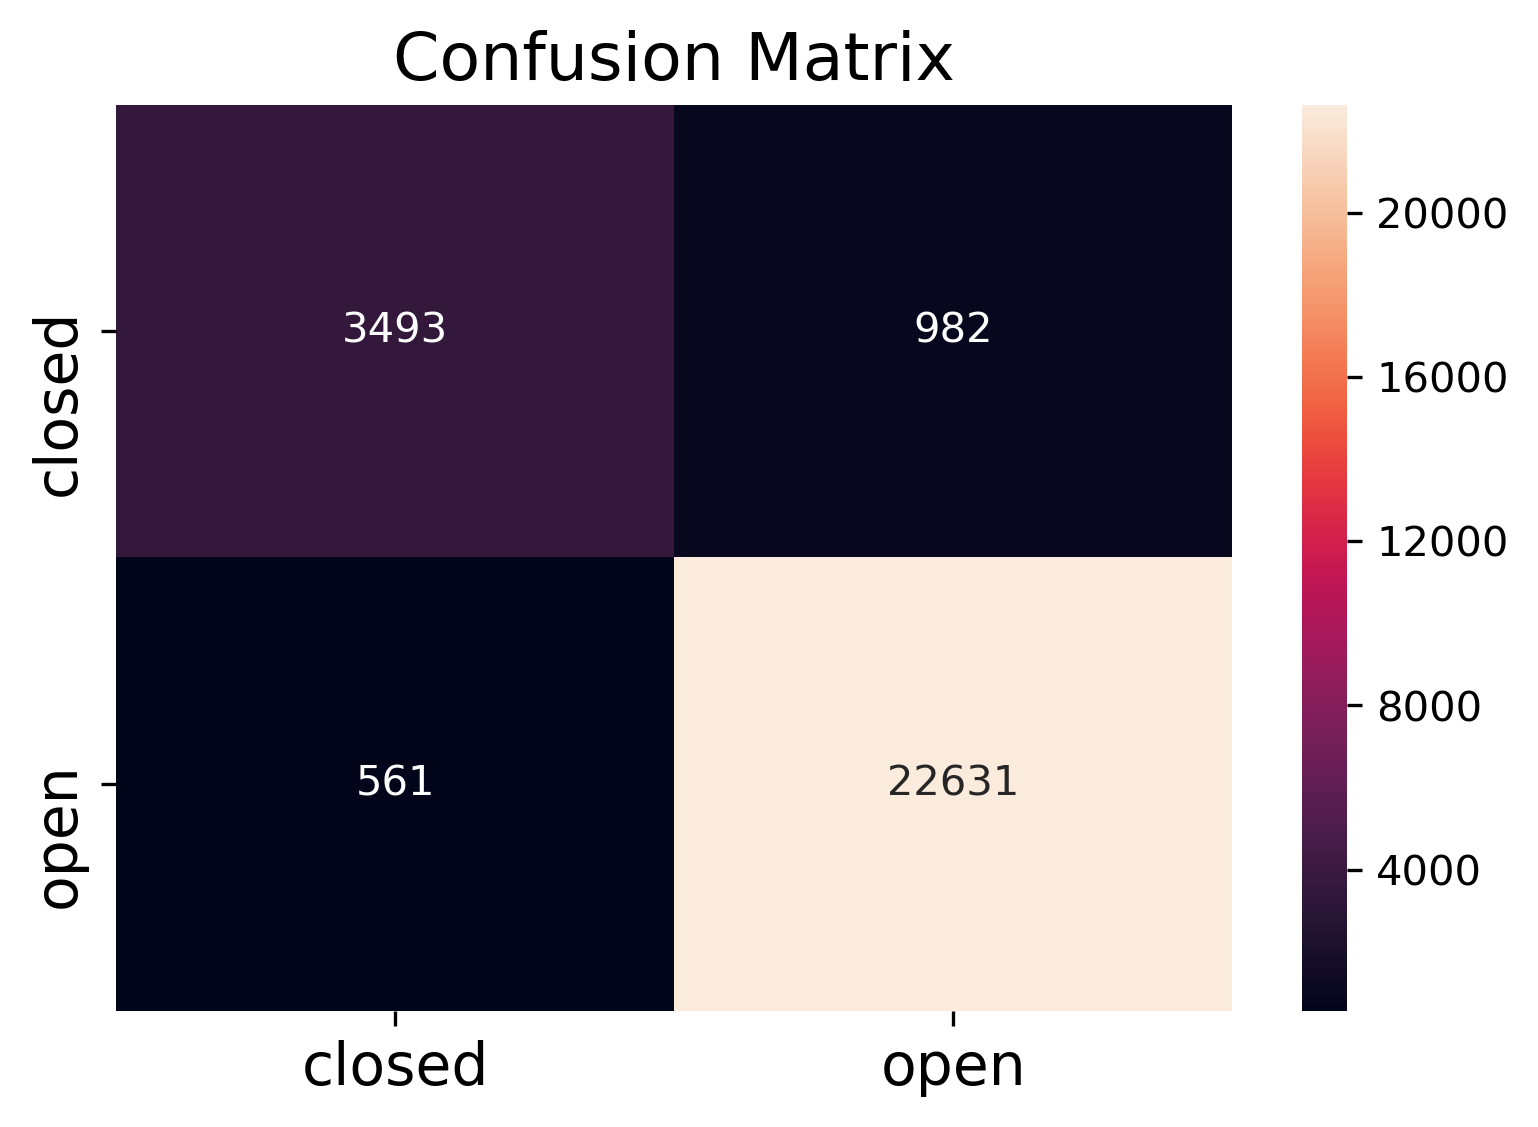
\includegraphics[width=.45\textwidth]{confusion}
\end{tabular} 
\end{tabular} 

As demonstrated above, the precision of open business is 96\% and closed business is 87\%. This means that among the businesses that are recognized as open by the model, 96\% of them actually remained open. The remaining 4\% are false positives. As to the closed businesses, 87\% are correctly recognized.\vspace{1em}

For a business investor, the interested factor could be the recall which includes the factor of how many businesses are actually closed but are not predicted as closed. 

\end{frame}
\subsection{Feature Importance}
\begin{frame}
\frametitle{Feature Importance}
\begin{figure}
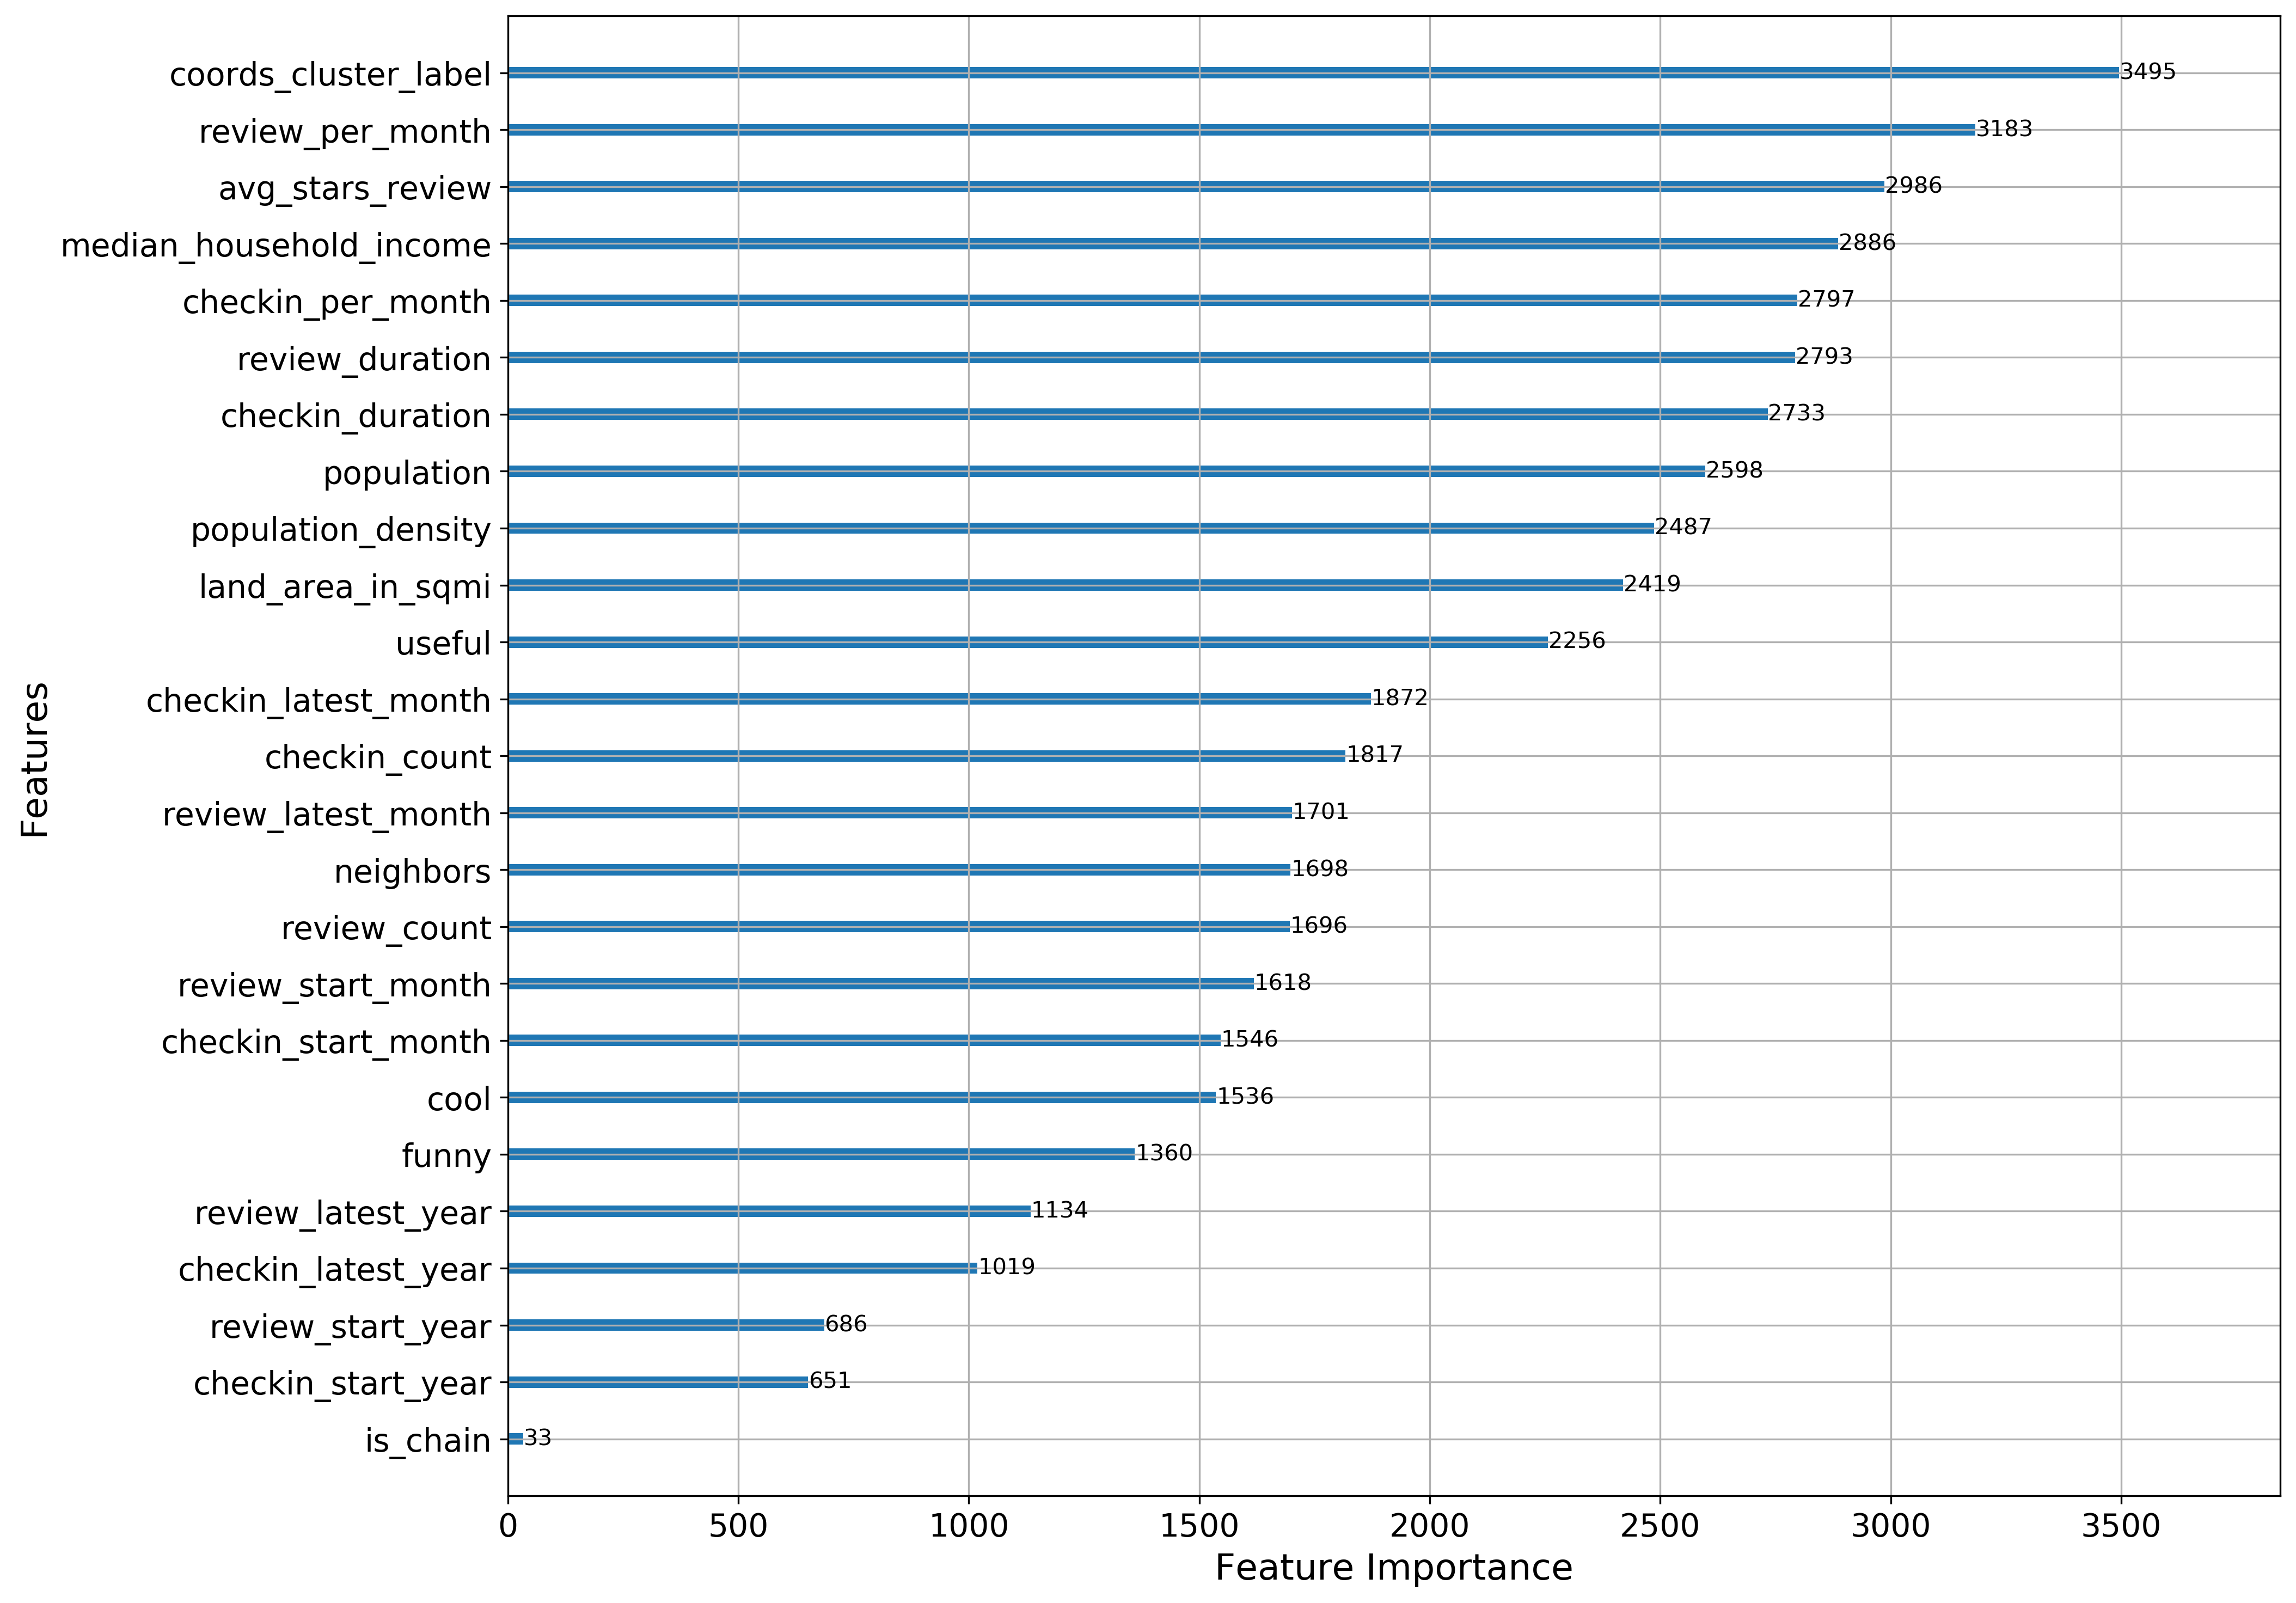
\includegraphics[width=\textwidth]{importance}
\end{figure}
\end{frame}

\begin{frame}
\frametitle{Feature Importance}
According to the feature importance that resulted from this model, following insights can be concluded:\vspace{1em}
\begin{itemize}
	\item The most important feature is the location clustering of the businesses
	\item Review rate, duration and stars also play essential roles
	\item Check-in factors which indicate how much effort a business is put on attracting customers are important as well
	\item The local residents' situation including income, population and density are crucial
\end{itemize}
These factors fit well with our common sense about if a business will success or not. In conclusion, the model performs well in predicting the status of a business.
\end{frame}
\subsection{Further Improvements}
\begin{frame}
\frametitle{Further Improvements}
Due to the imbalanced datasets, the training procedure tend to overfit the data after oversampling. The failure of a business is complicated, additional features could be taken into consideration to further improve the performance of the model:\vspace{1em}

\begin{itemize}
	\item Rental or housing price of the local area
	\item Price of the services
	\item Distinguish the type of a business (i.e. restaurant, SPA, bar, etc.)
	\item Analyze the review texts (NLP)
	\item Collect more data related to closed businesses
\end{itemize}
 
\end{frame}
%----------------------------------------------------------------------------------------
\section{Summary}
\begin{frame}
\frametitle{Summary}
\begin{itemize}
	\item Classify businesses in the US with Yelp's data into open and closed with lightGBM
	\item Review and check-in information are considered
	\item Information of local residents are introduced according to zipcode
	\item Businesses are clustered with latitude and longitude 
	\item An overall accuracy of 94.42\% is achieved
	\item Due to the imbalance of open and closed datasets, the model has higher variance on the closed businesses 
\end{itemize}
\end{frame}
%----------------------------------------------------------------------------------------

\end{document} 